\chapter{Использование кольцевого направленного ответвителя}

Кольцевой направленный ответвитель часто используется для создания суммарно-разностного сигнала, в том числе для балансных схем смесителей.

Соберём схему моделируемую схему (Рис.~\ref{fig:afd_homework_2_schematic}).

\begin{figure}[!ht]
    \centering
    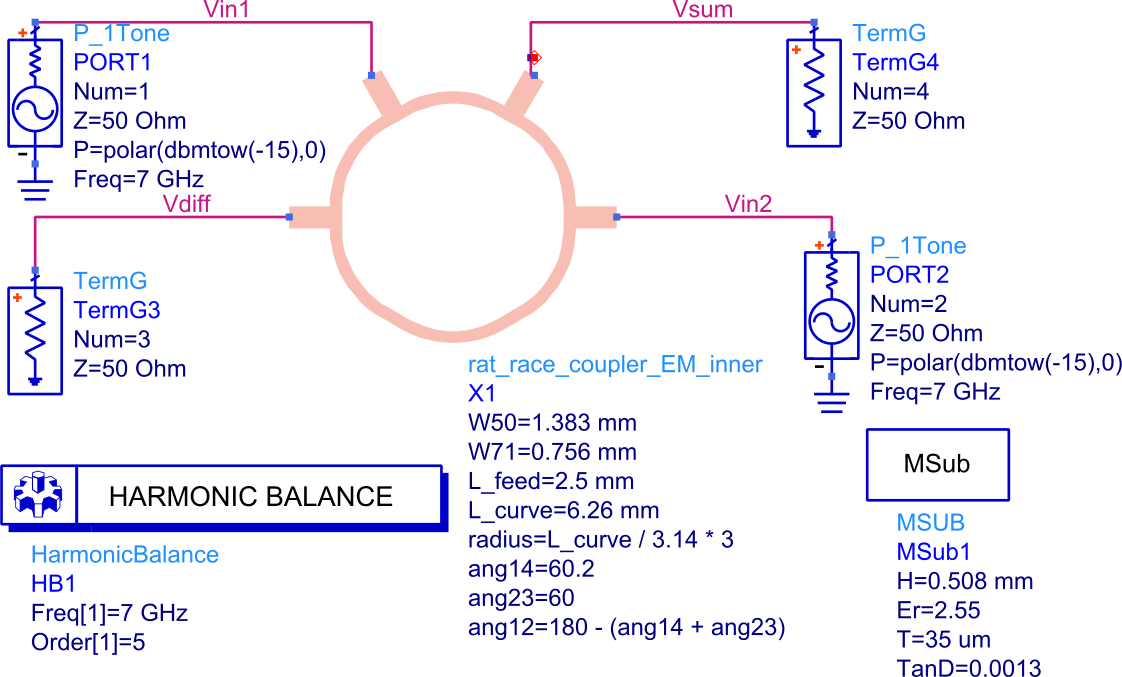
\includegraphics[width=\textwidth]{afd_homework_2_schematic.pdf}
    \caption{Балансный смеситель на основе кольцевого направленного ответвителя}%
    \label{fig:afd_homework_2_schematic}
\end{figure}

\section{Моделирование при подаче одинаковых сигналов}

Первым делом проведём моделирование при подаче сигналов с одинаковыми амплитудами и фазами.
Результат моделирования представлен на Рис.~\ref{fig:afd_homework_2_data_1}.

\begin{figure}[!ht]
    \centering
    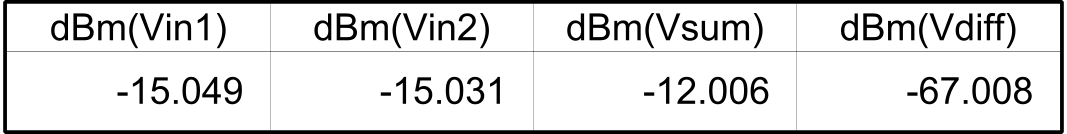
\includegraphics[width=0.5\textwidth]{afd_homework_2_data_1.pdf}
    \caption{}%
    \label{fig:afd_homework_2_data_1}
\end{figure}

На суммарный выход $V_\text{sum}$ приходит $-12~\text{дБм}$.
На разностный вывод $V_\text{diff}$ приходит $-67~\text{дБм}$, т.е. значение мощности близко к нулю.

\section{Моделирование при различных амплитудах}

Посмотрим на созвездие при типовой работе в смесителях: на вход опорного генератора поступает сигнал фиксированной мощности (пусть на вход $V_\text{in2}$ поступает сигнал мощностью $P = 10~\text{дБм}$ и фазой $45°$), а на вход $V_\text{in1}$ --- сигнал много меньшего уровня $P = -20~\text{дБм}$ и фазой $230^\circ$.

Изобразим созвездия на рабочей частоте $7~\text{ГГц}$.
Для получения данных в формате $\text{дБм}/{}^\circ$ для первой гармоники используем выражения, представленные на Рис.~\ref{fig:afd_homework_2_data_2_equations}.

\begin{figure}[!ht]
    \centering
    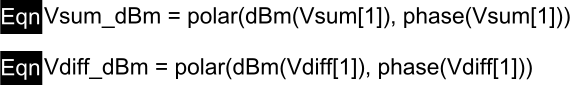
\includegraphics[width=0.5\textwidth]{afd_homework_2_data_2_equations.pdf}
    \caption{}%
    \label{fig:afd_homework_2_data_2_equations}
\end{figure}

Отобразим результат на графике в полярных координатах.

\begin{figure}[!ht]
    \centering
    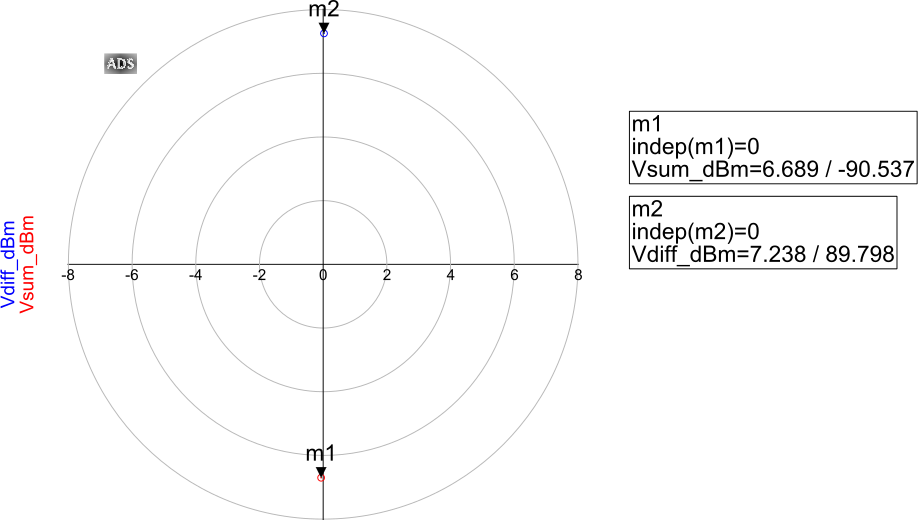
\includegraphics[width=0.7\textwidth]{afd_homework_2_data_2_minus_20_on_first.pdf}
    \caption{}%
    \label{fig:afd_homework_2_data_2_minus_20_on_first}
\end{figure}

Видно, что суммарный и разностный сигнал незначительно различаются по амплитуде и практически противоположны по фазе.

Уменьшим сигнал на входе $V_\text{in1}$ до $-30~\text{дБм}$.
Суммарно-разностный сигнал стал еще более симметричным.

\begin{figure}[!ht]
    \centering
    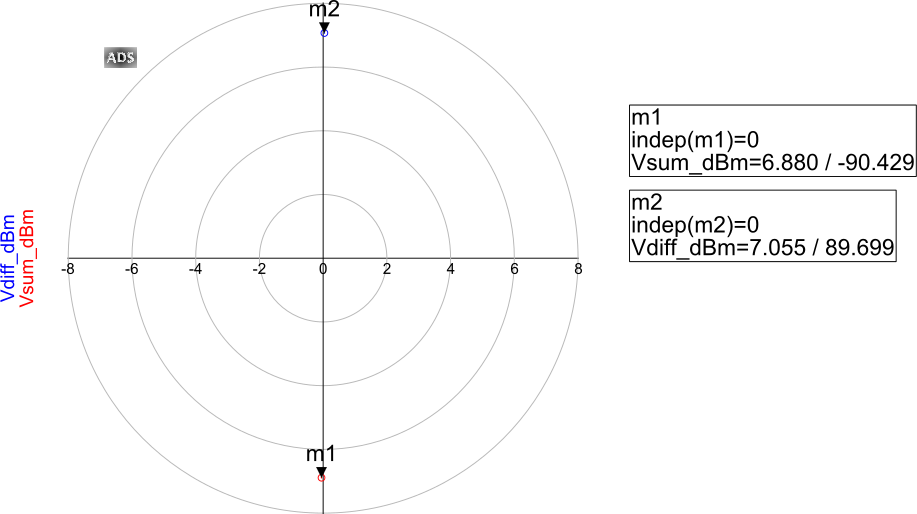
\includegraphics[width=0.7\textwidth]{afd_homework_2_data_2_minus_30_on_first.pdf}
    \caption{}%
    \label{fig:afd_homework_2_data_2_minus_30_on_first}
\end{figure}

\section{Моделирование при обратных значениях сигналов}

Поменяем местами сигналы на входах $V_\text{in1}$ и $V_\text{in2}$. $V_\text{sum}$ и $V_\text{diff}$ практически сливаются.

\begin{figure}[!ht]
    \centering
    \includegraphics[width=0.7\textwidth]{afd_homework_2_data_2_minus_20_on_second.pdf}
    \caption{}%
    \label{fig:afd_homework_2_data_2_minus_20_on_second}
\end{figure}
